%\usepackage[hyperref,table,x11names]{xcolor} % See documentation PDF at http://www.ctan.org/pkg/xcolor
\usetikzlibrary{matrix,arrows,positioning,automata,shadows,shapes.geometric,shapes.misc}
\definecolor{darkblue}{rgb}{.05,.05,.30}
\definecolor{darkgreen}{rgb}{.05,.30,.05}
\definecolor{darkred}{rgb}{.30,.05,.05}

\hspace*{-3em}%
 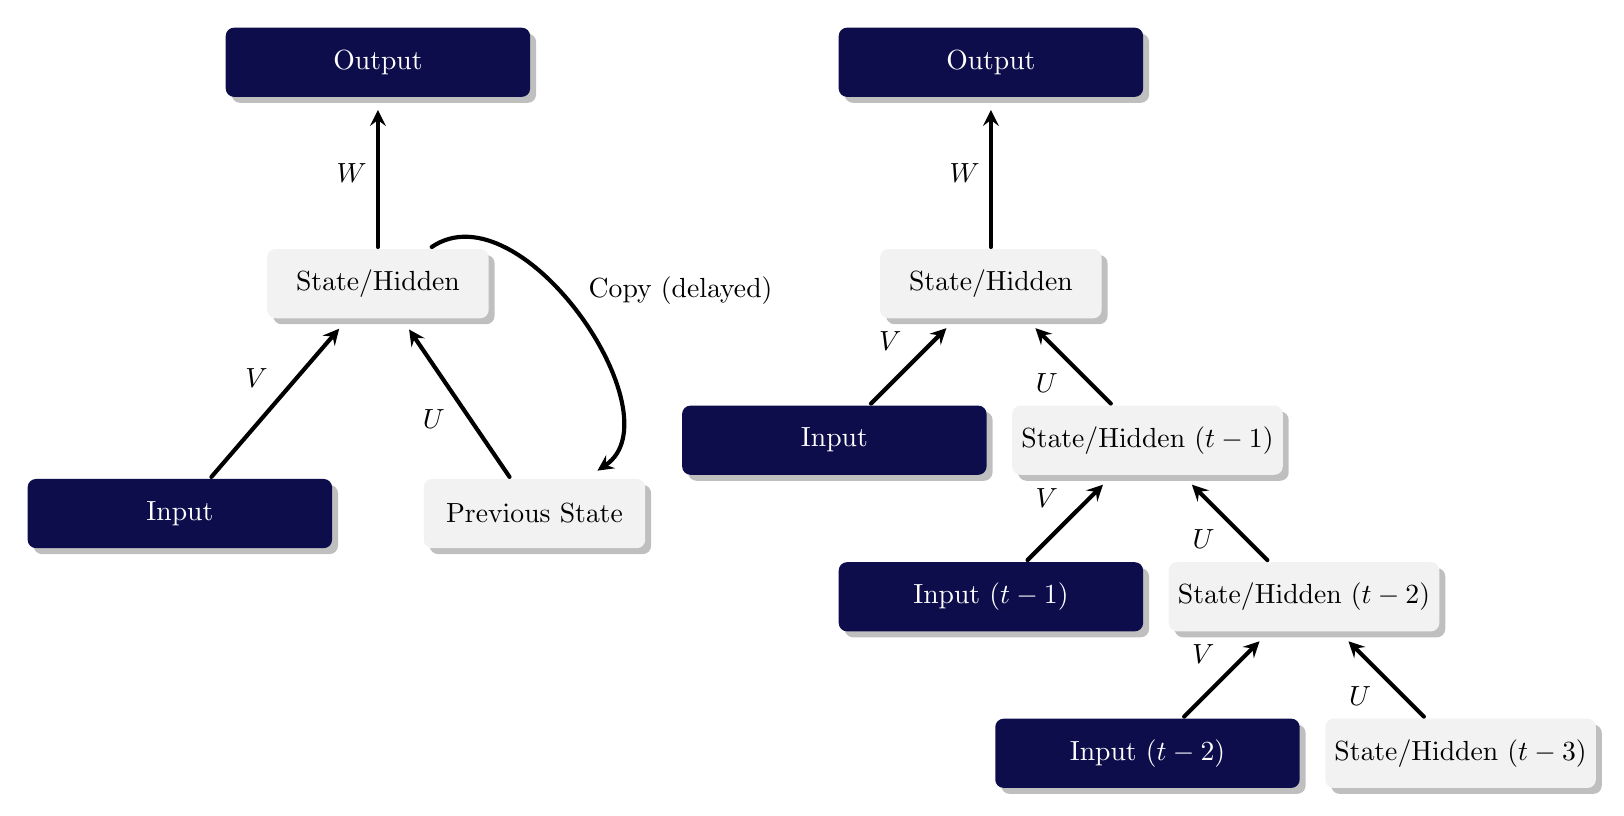
\begin{tikzpicture}[->, >=stealth, line cap=round, shorten >=.4em, auto, node distance=8.0em, semithick, initial text={},]
   \tikzstyle{every state}=[rounded corners=.3em, rectangle, fill=darkblue, draw=none, text=white, drop shadow, minimum width=11em, hidden/.style ={white!95!black,text=black,minimum width=8em},]
   \tikzstyle{every path}=[line width=.15em]

   \node[state] (output) {Output};
   \node[state,hidden] (hidden) [below of=output] {State/Hidden};
   \node[state] (input) [below left of=hidden] {Input};
   \node[state,hidden] (hidden_t-1) [below right of=hidden] {State/Hidden ($t-1$)};
   \node[state] (input_t-1) [below left of=hidden_t-1] {Input ($t-1$)};
   \node[state,hidden] (hidden_t-2) [below right of=hidden_t-1] {State/Hidden ($t-2$)};
   \node[state] (input_t-2) [below left of=hidden_t-2] {Input ($t-2$)};
   \node[state,hidden] (hidden_t-3) [below right of=hidden_t-2] {State/Hidden ($t-3$)};

   \node[state] (output_orig) [left=11.0em of output.west] {Output};
   \node[state,hidden] (hidden_orig) [below of=output_orig] {State/Hidden};
   \node[state] (input_orig) [below left=8em of hidden_orig.south east] {Input};
   \node[state,hidden] (previous) [below right=8em of hidden_orig.south west] {Previous State};


   \path

  (hidden)
    edge node {$W$} (output)
  (input)
    edge node {$V$} (hidden)
  (hidden_t-1)
    edge node {$U$} (hidden)
  (input_t-1)
    edge node {$V$} (hidden_t-1)
  (hidden_t-2)
    edge node {$U$} (hidden_t-1)
  (input_t-2)
    edge node {$V$} (hidden_t-2)
  (hidden_t-3)
    edge node {$U$} (hidden_t-2)

  (hidden_orig)
    edge [] node {$W$} (output_orig)
  (input_orig)
    edge [] node {$V$} (hidden_orig)
  (previous)
    edge [] node {$U$} (hidden_orig)
  (hidden_orig)
    edge [bend left=90] node {Copy (delayed)} (previous)
   ;
 \end{tikzpicture}